\chapter{Agujeros negros, agujeros blancos y el diagrama causal global}

\lectureoverview{Un horizonte es localmente ordinario y globalmente decisivo. Empezamos con la métrica de Schwarzschild cerca del horizonte, seguimos hacia el exterior mediante la analogía del cigarro euclídeo y, después, preguntamos qué pueden ver realmente Alice y Bob. La singularidad y la región de agujero blanco, que es la imagen temporal invertida, amplían ese cuadro local hasta abarcar el espacio-tiempo eterno de Schwarzschild. La compactificación de Penrose hace que la estructura causal sea finita y legible. Por último, pasamos de una solución eterna a un agujero negro formado por colapso, donde el teorema de la capa de Newton y el teorema de Birkhoff proporcionan las piezas que hay que empalmar.}

\section{Del horizonte al infinito}

Cerca del horizonte de Schwarzschild de un agujero suficientemente grande, la curvatura es débil en una región de laboratorio pequeña y la geometría radial-temporal es aproximadamente plana. La variable radial más conveniente no es la coordenada de Schwarzschild \(r\), sino la distancia propia \(\rho\) medida hacia el exterior desde el horizonte a lo largo de una hipersuperficie espacial de tiempo constante:
\begin{equation}
\rho=0 \quad\Longleftrightarrow\quad r=2GM .
\label{eq:l04-rho-horizon}
\end{equation}
La coordenada temporal más conveniente es la cantidad adimensional
\begin{equation}
\omega=\frac{t}{4GM},
\label{eq:l04-omega}
\end{equation}
donde \(c=1\). Así, \(\omega\) es el tiempo de Schwarzschild medido en unidades del doble del radio de Schwarzschild.

Con la convención de signos mayoritariamente positiva, la métrica radial-temporal cerca del horizonte es
\begin{equation}
ds^2\approx-\rho^2d\omega^2+d\rho^2.
\label{eq:l04-rindler}
\end{equation}
Se ha omitido la esfera angular bidimensional porque el argumento actual solo concierne al tiempo y a la distancia radial.

\begin{figure}[htbp]
\centering
\includegraphics[width=0.72\textwidth]{lecture_04_figure_02.png}
\caption{La métrica cerca del horizonte y el tiempo de Schwarzschild reescalado.}
\lectureframe{00:05:46.800}
\end{figure}

La ecuación~\eqref{eq:l04-rindler} guarda con el espacio-tiempo de Minkowski la misma relación que las coordenadas polares con el plano euclídeo. Para
\begin{equation}
T=\rho\sinh\omega,
\qquad
X=\rho\cosh\omega,
\end{equation}
se obtiene
\begin{equation}
-dT^2+dX^2=-\rho^2d\omega^2+d\rho^2.
\end{equation}
Las líneas de \(\rho\) constante son hipérbolas \(X^2-T^2=\rho^2\), mientras que \(\omega\) va del pasado remoto al futuro remoto. Las dos líneas nulas \(X=\pm T\) se encuentran en el punto de bifurcación del diagrama reducido. En cuatro dimensiones, ese punto representa una esfera bidimensional, y las hojas nulas futura y pasada forman un horizonte de Killing bifurcado.\editorialnote{En el diagrama radial, es útil llamar horizonte bifurcado solo al punto de intersección, como abreviatura. Más precisamente, las dos ramas del horizonte se intersectan en una esfera de bifurcación bidimensional.}

\subsection{La región lejana}

La parte radial-temporal de la métrica de Schwarzschild es
\begin{equation}
ds^2
=-\left(1-\frac{2GM}{r}\right)dt^2
+\frac{dr^2}{1-\frac{2GM}{r}}.
\label{eq:l04-schwarzschild}
\end{equation}
Lejos del agujero, \(r\gg2GM\), la métrica se aproxima a
\begin{equation}
ds^2\approx-dt^2+dr^2.
\end{equation}
Allí, \(r\) y \(\rho\) solo difieren en una corrección aditiva irrelevante, de modo que, con \(dt=4GM\,d\omega\),
\begin{equation}
ds^2\approx-(4GM)^2d\omega^2+d\rho^2.
\label{eq:l04-far}
\end{equation}
El coeficiente radial es sencillo en ambos límites. Lo que cambia es el coeficiente temporal:
\begin{equation}
ds^2\approx
\begin{cases}
-\rho^2d\omega^2+d\rho^2, & \rho\ll GM,\\[3pt]
-(4GM)^2d\omega^2+d\rho^2, & \rho\gg GM.
\end{cases}
\label{eq:l04-two-limits}
\end{equation}
A lo largo de una trayectoria estacionaria, \(d\rho=0\). Cerca del horizonte,
\begin{equation}
d\tau=\rho\,d\omega,
\end{equation}
mientras que, lejos de él, \(d\tau\approx4GM\,d\omega=dt\). Para un incremento fijo de la coordenada temporal exterior, transcurre cada vez menos tiempo propio en un reloj mantenido cada vez más cerca del horizonte.

\subsection{La cigarra}

Es difícil imaginar el espacio-tiempo, así que sustituyamos la dirección temporal por una dirección angular ordinaria. Escribamos
\begin{equation}
\begin{aligned}
d\ell^2&=F(\rho)^2d\theta^2+d\rho^2,\\
F(\rho)&\sim
\begin{cases}
\rho, & \rho\to0,\\
4GM, & \rho\to\infty.
\end{cases}
\end{aligned}
\label{eq:l04-cigar}
\end{equation}
Cerca de \(\rho=0\), esto es el plano en coordenadas polares. Lejos, la circunferencia deja de crecer con el radio:
\begin{equation}
C_\infty=\int_0^{2\pi}4GM\,d\theta=8\pi GM.
\label{eq:l04-cigar-circumference}
\end{equation}
Por tanto, la superficie se redondea en un extremo y se aproxima a un cilindro en el otro. Tiene aspecto de cigarra.

\begin{figure}[htbp]
\centering
\includegraphics[width=0.74\textwidth]{lecture_04_figure_03.png}
\caption{La comparación euclídea: una punta polar unida a un cilindro asintótico de circunferencia \(8\pi GM\).}
\lectureframe{00:14:05.000}
\end{figure}

Cuanto mayor es la masa, mayor es la cintura asintótica y más suave la curvatura cerca de la punta. Un agujero pequeño corresponde a una cigarra muy curvada; uno grande tiene una punta ancha y débilmente curvada. Esta imagen representa la interpolación de la ecuación~\eqref{eq:l04-two-limits}, no un embebimiento del propio agujero negro lorentziano.\editorialnote{El objeto geométrico preciso se obtiene continuando el tiempo de Schwarzschild a tiempo imaginario. La regularidad en la punta fija entonces el período del tiempo euclídeo en \(8\pi GM\), la misma escala que más adelante determina la temperatura de Hawking. Aquí, la clase solo utiliza la analogía visual.}

\section{Interpretación causal del horizonte}

Fuera del agujero, \(\rho>0\), un observador estacionario sigue una hipérbola de \(\rho\) constante. Lejos, basta una aceleración moderada para contrarrestar la gravedad; cerca del horizonte, la aceleración propia necesaria crece sin límite. Una vez que una línea de universo cruza la frontera nula futura, ninguna señal causal dirigida al futuro puede llegar desde ella hasta el exterior.

\begin{classroomqa}
\audiencequestion{¿Son rectas las trayectorias de los rayos de luz en este diagrama?\lecturetimestamp{00:20:21}}
\lecturerresponse{Los rayos de luz radiales se dibujan a \(45^\circ\), salvo que se indique otra convención. Un rayo entrante cruza el horizonte; un rayo saliente que ya está dentro no puede volver a cruzarlo hacia el exterior.}
\end{classroomqa}

\begin{classroomqa}
\audiencequestion{¿Permanece sobre el horizonte un rayo de luz entrante?\lecturetimestamp{00:21:12}}
\lecturerresponse{No. Un rayo dirigido hacia dentro cruza el horizonte futuro y continúa hacia el interior del agujero negro. Solo un generador del propio horizonte permanece en la frontera nula.}
\end{classroomqa}

\subsection{Bob observa a Alice}

Supongamos que Bob permanece suspendido en el exterior, a radio fijo, mientras Alice cae hacia dentro. Bob solo ve a Alice al recibir de ella luz que se propaga hacia el exterior. Supongamos que ella saluda periódicamente según su propio reloj. Las señales emitidas más tarde durante su caída tardan cada vez más tiempo de Schwarzschild en llegar a Bob, y él recibe menos ondas por unidad de tiempo. Ninguna señal emitida después de que ella cruce el horizonte puede volver hasta él.

Las coordenadas de Rindler muestran el comportamiento límite. Definamos la coordenada nula saliente
\begin{equation}
U=T-X=-\rho e^{-\omega}.
\end{equation}
Acercarse al horizonte futuro significa que \(U\to0^{-}\), lo que requiere que \(\omega\to+\infty\) para un valor fijo de \(\rho\) exterior. Por tanto, un evento de cruce finito para Alice queda desplazado a un tiempo exterior infinito. Las crestas sucesivas de las ondas llegan cada vez más separadas, de modo que su frecuencia experimenta un corrimiento al rojo exponencial.\editorialnote{Este cálculo con coordenadas nulas da la forma matemática del corrimiento al rojo que se describió cualitativamente en clase. Solo utiliza la aproximación local de Rindler.}

Al principio Bob recibe luz visible; después, infrarroja y, más tarde, ondas de radio de longitud de onda enorme. Lo útil no es decir que Alice permanece como una fotografía permanentemente visible sobre el horizonte. Se vuelve más tenue y más roja, hasta que finalmente deja de ser detectable.

\begin{classroomqa}
\audiencequestion{¿Ve Bob a Alice congelada en un punto exacto fuera del horizonte?\lecturetimestamp{00:26:31}}
\lecturerresponse{En la descripción clásica con coordenadas exteriores, las imágenes que recibe cada vez más tarde proceden de eventos cada vez más próximos al horizonte. La imagen límite queda congelada allí, pero su radiación sufre un corrimiento al rojo hasta que, en la práctica, desaparece. Esta explicación todavía no incluye la física cuántica de los agujeros negros.}
\end{classroomqa}

\begin{classroomqa}
\audiencequestion{A medida que Alice se desvanece, ¿también parece comprimirse?\lecturetimestamp{00:28:34}}
\lecturerresponse{Sí. El movimiento relativo produce una contracción de Lorentz longitudinal en la descripción exterior. El efecto observacional importante sigue siendo el corrimiento al rojo: sus oscilaciones internas parecen más lentas y la longitud de onda recibida aumenta.}
\end{classroomqa}

\subsection{Alice observa a Bob}

El tiempo propio de Alice sigue siendo regular en el horizonte. Después de cruzarlo, continúa recibiendo señales de Bob que se propagan hacia dentro, porque esas señales siguen la misma dirección causal que ella. Una vez dentro, no puede responder al exterior. El horizonte es unidireccional, no una pared que se encuentre de forma simétrica desde ambos lados.

\begin{classroomqa}
\audiencequestion{¿Ve Alice con corrimiento al azul la luz de Bob mientras cae y atraviesa el horizonte?\lecturetimestamp{00:30:29}}
\lecturerresponse{En la imagen que estamos usando, Alice ve a Bob alejarse y sus señales desplazarse hacia el rojo; nada singular ocurre cuando ella cruza. El corrimiento preciso de la frecuencia depende de ambas líneas de universo y del momento en que emite Bob, así que la afirmación invariante es que la frecuencia medida por Alice permanece finita en un horizonte regular.}
\end{classroomqa}

\begin{classroomqa}
\audiencequestion{¿Se aplica la misma restricción causal a los gravitones?\lecturetimestamp{00:31:15}}
\lecturerresponse{Se aplica a la radiación gravitatoria genuina igual que a los fotones. Ninguna perturbación radiativa emitida detrás del horizonte futuro puede llegar hasta Bob.}
\end{classroomqa}

\begin{classroomqa}
\audiencequestion{Cuando Alice cae dentro, ¿su energía aumenta la masa y el radio del agujero?\lecturetimestamp{00:31:43}}
\lecturerresponse{Sí. Cuando su energía queda incluida en el agujero negro, su masa aumenta y el radio de Schwarzschild \(R_s=2GM\) aumenta con ella. El problema de formación dinámica dará contenido geométrico a esta afirmación.}
\end{classroomqa}

\subsection{Por qué el exterior sigue teniendo gravedad}

Un agujero negro es oscuro, pero no carece de gravedad. Un campo gravitatorio estacionario no es un flujo de gravitones reales que escapen continuamente del interior. Es la geometría exterior ya establecida. Si cambia la fuente, el cambio del campo se propaga causalmente; un observador distante no puede detectar ese cambio antes de que pudiera llegarle una señal luminosa.

\begin{classroomqa}
\audiencequestion{Si los gravitones no pueden escapar, ¿por qué ejerce gravedad el agujero negro?\lecturetimestamp{00:32:04}}
\lecturerresponse{El campo estático ya está presente en el exterior. Puede describirse informalmente mediante gravitones virtuales, pero estos no son partículas detectables que transporten mensajes nuevos desde el interior. Lo que está limitado por la velocidad de la luz es cualquier cambio del campo, incluida la radiación gravitatoria.}
\end{classroomqa}

\begin{classroomqa}
\audiencequestion{¿Cómo se concilia la idea de gravitones virtuales con la afirmación de que un cambio del campo se propaga a la velocidad de la luz?\lecturetimestamp{00:34:02}}
\lecturerresponse{Los cuantos virtuales son elementos contables de un cálculo perturbativo, no partículas portadoras de señales con trayectorias medibles. Las perturbaciones invariantes gauge y la información se propagan causalmente. La misma distinción existe entre un campo electromagnético estático y la radiación electromagnética.}
\end{classroomqa}

Por tanto, no debe entenderse que la afirmación de clase de que los gravitones virtuales pueden superar la velocidad de la luz implique una comunicación superlumínica.\editorialnote{Las partículas virtuales fuera de la capa de masa no tienen que satisfacer la relación de dispersión de las partículas reales, pero no son observables ni pueden utilizarse para transmitir información. En relatividad general, la descripción es más sencilla y clara: la métrica exterior estacionaria existe, mientras que los cambios del campo gravitatorio se propagan causalmente.}

\section{¿Puede Alice seguir viendo sus pies?}

Supongamos que Alice cae con los pies por delante. Sus pies cruzan el horizonte antes que su cabeza. Cuando mira hacia abajo, nunca ve el evento simultáneo en la línea de universo de sus pies; la luz tarda en viajar, así que los ve en un evento ligeramente anterior. Existe una sucesión continua de esos eventos pasados antes y después de que su cabeza cruce. El mero hecho de que una parte de su cuerpo haya pasado \(r=2GM\) no produce ninguna discontinuidad local.

El experimento peligroso consiste en cambiar de rumbo cuando los pies ya están dentro. Para mantener la cabeza fuera, Alice debe acelerarse hacia el exterior. Sus pies, que ya han atravesado el horizonte futuro, no pueden seguir una trayectoria estacionaria en el exterior. La separación en el sistema acelerado crece sin límite, y un cuerpo material no puede permanecer rígido a ambos lados de esa frontera causal. Alice debe caer libremente con los pies o ser despedazada al intentar mantener fuera el resto del cuerpo.

Este estiramiento no se debe a una fuerza de marea divergente en un horizonte grande. Es consecuencia de exigir líneas de universo incompatibles para un cuerpo extenso.\editorialnote{Un horizonte de Schwarzschild suficientemente grande tiene una curvatura de marea pequeña. La patología de este experimento mental se debe al intento de imponer aceleración y rigidez, no a una singularidad local de la curvatura en el horizonte.}

\section{La singularidad está en el futuro}

Volvamos a la ecuación~\eqref{eq:l04-schwarzschild}. En el exterior,
\begin{equation}
1-\frac{2GM}{r}>0,
\end{equation}
de modo que \(t\) es temporal y \(r\) espacial en las coordenadas de Schwarzschild. En el interior,
\begin{equation}
1-\frac{2GM}{r}<0,
\end{equation}
y esos papeles coordinados se invierten: disminuir \(r\) es una dirección temporal. Esto no significa que el espacio se convierta físicamente en tiempo en el horizonte. Significa que la carta de Schwarzschild se degenera allí y que sus coordenadas tienen distinto carácter causal en el interior.

La singularidad verdadera se encuentra en
\begin{equation}
r=0.
\end{equation}
No es una línea de universo vertical que represente un lugar que se pueda evitar. Es una frontera futura de tipo espacial. Una vez que Alice entra en la región del agujero negro, toda trayectoria futura de tipo temporal o nulo termina allí. El invariante de curvatura
\begin{equation}
R_{\mu\nu\rho\sigma}R^{\mu\nu\rho\sigma}
=\frac{48G^2M^2}{r^6}
\label{eq:l04-kretschmann}
\end{equation}
diverge cuando \(r\to0\), mientras que es finito en \(r=2GM\).\editorialnote{La ecuación~\eqref{eq:l04-kretschmann} es el escalar de Kretschmann habitual de Schwarzschild. Expresa de forma invariante la distinción geométrica trazada en la clase entre el horizonte regular y la singularidad de curvatura.}

\section{Inversión temporal y agujero blanco}

La métrica de Schwarzschild es independiente de \(t\), y \(dt^2\) permanece inalterado bajo \(t\mapsto-t\). Por tanto, su extensión máxima es simétrica bajo inversión temporal. Junto con la singularidad y el horizonte futuros, la solución matemática contiene una singularidad pasada y un horizonte pasado.

Invirtamos temporalmente la caída de Alice. Ahora emerge de la singularidad pasada, cruza hacia fuera el horizonte pasado y aparece en el exterior de Bob. Esa región se llama agujero blanco. No es una vía de escape desde el interior del agujero negro futuro: los horizontes futuro y pasado son fronteras nulas distintas.

\begin{classroomqa}
\audiencequestion{Si Alice no puede cruzar hacia fuera el horizonte del agujero negro, ¿cómo puede salir la Alice con el tiempo invertido?\lecturetimestamp{00:50:24}}
\lecturerresponse{No cruza hacia fuera el horizonte futuro. Cruza hacia fuera el horizonte pasado, exactamente como ocurre en la inversión temporal de una caída ordinaria. La región del agujero negro futuro sigue sin tener ninguna trayectoria causal saliente.}
\end{classroomqa}

\begin{classroomqa}
\audiencequestion{En la imagen del agujero blanco, ¿también hay que invertir el sentido temporal de toda la historia de Bob?\lecturetimestamp{00:52:15}}
\lecturerresponse{No. La geometría extendida admite una historia en la que Bob permanece en el exterior mientras Alice emerge del horizonte pasado. El problema no es la coherencia matemática, sino la condición inicial extraordinaria que representa la singularidad pasada.}
\end{classroomqa}

\begin{figure}[htbp]
\centering
\includegraphics[width=0.72\textwidth]{lecture_04_figure_04.png}
\caption{Esquema causal desarrollado: horizontes que se cruzan, curvas de singularidad futura y pasada, y trayectorias de observadores añadidas a lo largo del análisis.}
\lectureframe{01:00:19.818}
\end{figure}

\begin{figure}[htbp]
\centering
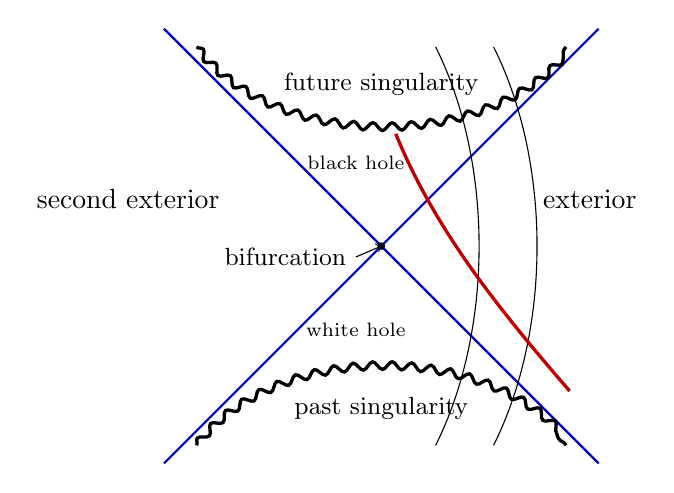
\begin{tikzpicture}[scale=0.92]
\draw[blue!75!black,thick] (-3,-3) -- (3,3);
\draw[blue!75!black,thick] (-3,3) -- (3,-3);
\draw[very thick,decorate,decoration={snake,amplitude=1.4pt,segment length=7pt}]
  (-2.55,2.75) .. controls (-1.45,1.35) and (1.45,1.35) .. (2.55,2.75);
\draw[very thick,decorate,decoration={snake,amplitude=1.4pt,segment length=7pt}]
  (-2.55,-2.75) .. controls (-1.45,-1.35) and (1.45,-1.35) .. (2.55,-2.75);
\draw (0.75,-2.75) .. controls (1.55,-1.15) and (1.55,1.15) .. (0.75,2.75);
\draw (1.55,-2.75) .. controls (2.35,-1.15) and (2.35,1.15) .. (1.55,2.75);
\draw[red!75!black,very thick] (2.6,-2.0) .. controls (1.65,-0.9) and (0.75,0.2) .. (0.2,1.55);
\fill (0,0) circle (1.5pt);
\node[above,font=\small] at (0,1.95) {future singularity};
\node[below,font=\small] at (0,-1.95) {past singularity};
\node[right] at (2.10,0.65) {exterior};
\node[left] at (-2.10,0.65) {second exterior};
\node[font=\scriptsize] at (-0.35,1.15) {black hole};
\node[font=\scriptsize] at (-0.35,-1.15) {white hole};
\node[font=\small,anchor=east] (bifurcation-label) at (-0.35,-0.15) {bifurcation};
\draw[->,thin] (bifurcation-label.east) -- (0,0);
\end{tikzpicture}
\caption{Diagrama causal sin compactificar, ya limpio. Los horizontes nulos se cruzan en la superficie de bifurcación; las singularidades de tipo espacial se encuentran en las regiones futura y pasada.}
\end{figure}

\subsection{Posible no significa típico}

La mecánica microscópica es invariante bajo inversión temporal con excelente aproximación, pero las historias macroscópicas tienen una dirección preferente. Una bomba explota con facilidad; casi nunca vuelven a reunirse los fragmentos dispersos para reconstruirla. Una pelota rueda fácilmente desde una cima inestable; casi nunca una pelota lanzada al azar se detiene exactamente allí. Las bolas de billar colocadas en un triángulo se dispersan con facilidad, mientras que las bolas dispersas no se ordenan espontáneamente para formar el triángulo. Un cubo de hielo se derrite en agua caliente, mientras que el agua casi nunca expulsa un cubo de hielo recién formado.

La distinción es la entropía. Un macroestado de baja entropía ocupa una región diminuta del espacio de fases; un macroestado de alta entropía comprende una cantidad enorme de configuraciones microscópicas. Las ecuaciones permiten la trayectoria inversa, pero preparar su microestado inicial exige correlaciones de una precisión extraordinaria.

\begin{classroomqa}
\audiencequestion{¿Acaso cada configuración dispersa exacta no es tan improbable como la configuración exacta con el tiempo invertido?\lecturetimestamp{00:56:55}}
\lecturerresponse{Sí, si se trata de microestados especificados individualmente. La asimetría aparece al comparar macroestados. Una configuración dispersa comprende muchísimos más microestados que un triángulo ensamblado con precisión, así que casi todo microestado compatible con la primera descripción sigue estando desordenado a escala macroscópica.}
\end{classroomqa}

Un agujero blanco que emite una Alice completamente organizada es la versión gravitatoria de una historia en la que disminuye la entropía. Las ecuaciones reversibles la permiten, pero exige un pasado extraordinariamente especial. El horizonte mismo tiene entropía e información microscópica oculta, así que una fluctuación del tamaño de Alice no está prohibida lógicamente, aunque su probabilidad queda abrumadoramente suprimida.

\begin{classroomqa}
\audiencequestion{¿Sería una fluctuación de este tipo cuántica o térmica?\lecturetimestamp{00:59:48}}
\lecturerresponse{Pueden contribuir ambos tipos. En un sistema caliente ordinario, la descripción predominante es la de una fluctuación térmica; en un agujero negro, los efectos cuánticos y térmicos están entrelazados. En cualquier caso, la supresión fundamental es entrópica.}
\end{classroomqa}

\section{Distancia propia y compactificación de Penrose}

Antes de dibujar el espacio-tiempo global, conviene precisar la terminología radial. El tiempo propio es lo que mide un reloj a lo largo de una línea de universo de tipo temporal. La distancia propia es lo que mide una cadena de reglas locales a lo largo de una curva espacial elegida. Para la hipersuperficie de Schwarzschild a \(t\) constante,
\begin{equation}
d\rho=\frac{dr}{\sqrt{1-2GM/r}}.
\label{eq:l04-proper-distance}
\end{equation}
Así, \(r\) es una coordenada areal, no la distancia directa desde el horizonte medida con reglas.

Empecemos ahora con el espacio-tiempo radial plano. Conservemos solo \(t\) y \(\rho\ge0\). La línea \(\rho=0\) es el origen espacial, y un rayo de luz radial que entra en el origen continúa hacia fuera por el lado físico opuesto, lo que aparece como una reflexión en el semiplano reducido.

Un diagrama de Penrose transforma todos los valores finitos e infinitos de \(t\) y \(\rho\) en una región finita, conservando las direcciones nulas. Sus dos reglas son:
\begin{enumerate}
\item compactar todo el espacio-tiempo en un dominio finito;
\item mantener los rayos de luz radiales a \(45^\circ\).
\end{enumerate}
Las longitudes y los ángulos ordinarios se distorsionan; las relaciones causales, no.

\begin{figure}[htbp]
\centering
\includegraphics[width=0.70\textwidth]{lecture_04_figure_06.png}
\caption{La retícula completa de la compactificación del espacio-tiempo de Minkowski radial. El tiempo infinito queda en los extremos superior e inferior izquierdos, y el radio infinito se comprime hasta la punta derecha.}
\lectureframe{01:14:44.040}
\end{figure}

\begin{figure}[htbp]
\centering
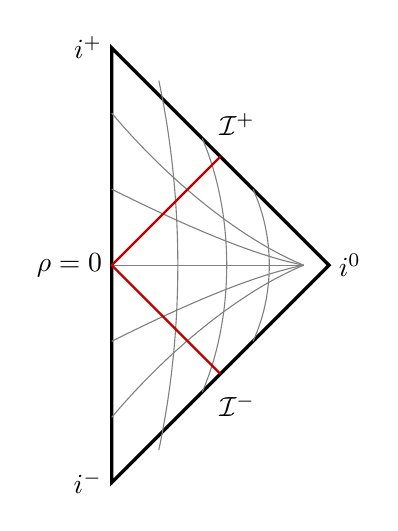
\begin{tikzpicture}[scale=0.92]
\coordinate (im) at (0,-3);
\coordinate (ip) at (0,3);
\coordinate (iz) at (3,0);
\draw[very thick] (im) -- (ip) -- (iz) -- cycle;
\draw[gray] (0,-2.1) .. controls (0.8,-1.15) and (1.8,-0.35) .. (2.65,0);
\draw[gray] (0,-1.05) .. controls (0.9,-0.6) and (1.9,-0.15) .. (2.65,0);
\draw[gray] (0,0) -- (2.65,0);
\draw[gray] (0,1.05) .. controls (0.9,0.6) and (1.9,0.15) .. (2.65,0);
\draw[gray] (0,2.1) .. controls (0.8,1.15) and (1.8,0.35) .. (2.65,0);
\draw[gray] (0.65,-2.55) .. controls (1.0,-0.9) and (1.0,0.9) .. (0.65,2.55);
\draw[gray] (1.25,-1.75) .. controls (1.7,-0.7) and (1.7,0.7) .. (1.25,1.75);
\draw[gray] (1.95,-1.05) .. controls (2.25,-0.4) and (2.25,0.4) .. (1.95,1.05);
\draw[red!75!black,thick] (1.5,-1.5) -- (0,0) -- (1.5,1.5);
\node[left] at (ip) {\(i^+\)};
\node[left] at (im) {\(i^-\)};
\node[right] at (iz) {\(i^0\)};
\node[above right] at (1.35,1.65) {\(\mathcal{I}^+\)};
\node[below right] at (1.35,-1.65) {\(\mathcal{I}^-\)};
\node[left] at (0,0) {\(\rho=0\)};
\end{tikzpicture}
\caption{El espacio-tiempo de Minkowski radial en un triángulo finito. El rayo nulo rojo entra desde \(\mathcal{I}^-\), llega al origen y sale por \(\mathcal{I}^+\).}
\label{fig:l04-flat-penrose}
\end{figure}

Los extremos tienen significados causales distintos:
\begin{equation}
\begin{aligned}
i^-&:\ \text{past timelike infinity},\\
i^+&:\ \text{future timelike infinity},\\
i^0&:\ \text{spatial infinity},\\
\mathcal{I}^-&:\ \text{past null infinity},\\
\mathcal{I}^+&:\ \text{future null infinity}.
\end{aligned}
\end{equation}
Los símbolos \(\mathcal{I}^{-}\) y \(\mathcal{I}^{+}\) se pronuncian «scri menos» y «scri más».

\begin{classroomqa}
\audiencequestion{¿Debería un rayo nulo pasar por las esquinas de cada celda deformada de la retícula y, por tanto, curvarse ligeramente?\lecturetimestamp{01:11:08}}
\lecturerresponse{Si se dibujara con exactitud toda la retícula de coordenadas, sus intersecciones serían compatibles con la curva nula. La construcción esencial es conforme: las direcciones nulas radiales siguen formando un ángulo de \(45^\circ\), aunque las líneas de \(t\) y \(\rho\) constantes se curven y se agrupen.}
\end{classroomqa}

\begin{classroomqa}
\audiencequestion{¿Cómo se dibuja un rayo de luz si no pasa por el origen?\lecturetimestamp{01:11:45}}
\lecturerresponse{Llega a una distancia mínima no nula y vuelve hacia fuera. Al incluir el movimiento angular, su trayectoria radial proyectada no tiene por qué ser una única línea recta a \(45^\circ\).}
\end{classroomqa}

\begin{classroomqa}
\audiencequestion{Entonces, ¿por qué ese rayo de luz no está a \(45^\circ\)?\lecturetimestamp{01:12:49}}
\lecturerresponse{La regla de \(45^\circ\) se enunció para los rayos de luz radiales. Un rayo nulo con momento angular utiliza parte de su movimiento en las direcciones angulares, de modo que su proyección sobre el plano \(t\)-\(\rho\) no es radial.}
\end{classroomqa}

\section{El diagrama de Schwarzschild eterno}

El diagrama compactificado tiene cuatro regiones. Sus dos rombos laterales son exteriores asintóticamente planos. El triángulo superior es el interior del agujero negro y termina en la singularidad futura de tipo espacial. El triángulo inferior es la región del agujero blanco y comienza en la singularidad pasada de tipo espacial. En conjunto, estas regiones forman la geometría de Schwarzschild extendida al máximo.

\begin{figure}[htbp]
\centering
\includegraphics[width=0.74\textwidth]{lecture_04_figure_07.png}
\caption{El diagrama de Penrose completo de Schwarzschild eterno, con las singularidades, los horizontes, las trayectorias nulas y una frontera asintótica señalados en la pizarra.}
\lectureframe{01:21:30.000}
\end{figure}

\begin{figure}[htbp]
\centering
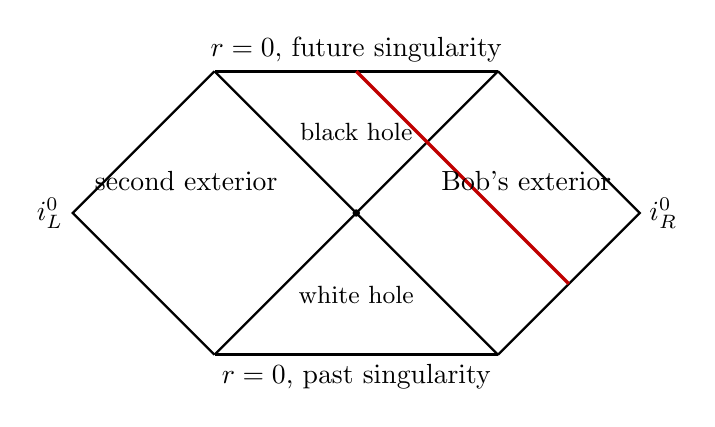
\begin{tikzpicture}[scale=0.90]
\coordinate (C) at (0,0);
\coordinate (TL) at (-2,2);
\coordinate (TR) at (2,2);
\coordinate (BL) at (-2,-2);
\coordinate (BR) at (2,-2);
\coordinate (L) at (-4.0,0);
\coordinate (R) at (4.0,0);
\draw[very thick] (TL) -- (TR);
\draw[very thick] (BL) -- (BR);
\draw[thick] (C) -- (TL) (C) -- (TR) (C) -- (BL) (C) -- (BR);
\draw[thick] (TL) -- (L) -- (BL);
\draw[thick] (TR) -- (R) -- (BR);
\draw[red!75!black,very thick] (3,-1) -- (1,1) -- (0,2);
\node[above] at (0,2) {\(r=0\), future singularity};
\node[below] at (0,-2) {\(r=0\), past singularity};
\node[font=\small] at (0,1.15) {black hole};
\node[font=\small] at (0,-1.15) {white hole};
\node at (2.4,0.45) {Bob's exterior};
\node at (-2.4,0.45) {second exterior};
\node[right] at (R) {\(i^0_R\)};
\node[left] at (L) {\(i^0_L\)};
\fill (C) circle (1.5pt);
\end{tikzpicture}
\caption{Las cuatro regiones de Schwarzschild eterno. Un rayo de luz radial entrante cruza el horizonte futuro y termina en \(r=0\).}
\label{fig:l04-eternal}
\end{figure}

Un rayo de luz radial entrante desde \(\mathcal{I}^-\) cruza el horizonte futuro y termina en la singularidad. Todas las curvas causales del triángulo superior comparten ese destino. A menudo se describe el segundo exterior como la otra boca de un puente de Einstein--Rosen, pero no es transitable: cualquier intento de viaje causal de un exterior al otro entra en la región del agujero negro y llega a la singularidad.

\begin{classroomqa}
\audiencequestion{¿Están conectados los dos mundos exteriores por un agujero de gusano, y se puede enviar una señal a través de él?\lecturetimestamp{01:22:21}}
\lecturerresponse{La geometría eterna contiene un puente de Einstein--Rosen en ciertas hipersuperficies espaciales, pero ninguna señal causal cruza de un exterior al otro. El puente se cierra demasiado deprisa; incluso la luz que entra en un horizonte termina en la singularidad futura.}
\end{classroomqa}

Este diagrama describe un agujero que ha existido desde siempre. Los agujeros astrofísicos reales se forman a partir de materia en colapso. Su diagrama causal no tiene una singularidad pasada de agujero blanco ni un segundo exterior asintótico. Para construir esa geometría, tenemos que entender las capas esféricas.

\section{Formación de un agujero negro por colapso}

Imaginemos una capa esférica difusa de partículas entrantes. Pueden ser fotones: la energía gravita, así que un pulso de radiación suficientemente concentrado puede formar un agujero negro. Antes del colapso, la región central se parece al espacio-tiempo plano vacío; una vez comprimida suficiente energía, el exterior se parece al espacio-tiempo de Schwarzschild. La tarea consiste en empalmar esas regiones a través de la capa en movimiento.

\subsection{Teorema de la capa de Newton}

Para una capa newtoniana esférica simétrica de masa total \(M\), la ley de Gauss para la gravedad es
\begin{equation}
\oint \mathbf{g}\cdot d\mathbf{A}=-4\pi G M_{\mathrm{enc}}.
\label{eq:l04-gauss-gravity}
\end{equation}
La simetría esférica implica que \(\mathbf{g}=g(r)\hat{\mathbf r}\), así que
\begin{equation}
g(r)=
\begin{cases}
0, & r<R_{\mathrm{shell}},\\[4pt]
-\dfrac{GM}{r^2}, & r>R_{\mathrm{shell}}.
\end{cases}
\label{eq:l04-shell-field}
\end{equation}
En el interior no hay masa encerrada y el campo gravitatorio se anula. En el exterior, la capa actúa exactamente como una masa puntual \(M\) situada en el centro. El potencial en el interior es constante, aunque no nulo, pero no queda ninguna fuerza newtoniana local.\editorialnote{El argumento basado en las líneas de campo que se expuso en clase queda expresado con precisión por la ley de Gauss. La distinción entre campo nulo y potencial constante importa al comparar las normalizaciones de los relojes en relatividad.}

La conclusión sigue siendo válida mientras se contraiga una capa perfectamente esférica, siempre que su masa total se conserve. Solo cambia la ubicación de la frontera entre las soluciones interior y exterior.

\subsection{Teorema de Birkhoff}

El análogo relativista es el teorema de Birkhoff: toda región de vacío con simetría esférica es localmente una porción de la familia de Schwarzschild. Para una capa sin masa en su centro,
\begin{align}
ds^2_{\mathrm{inside}}&=-dT^2+dR^2+R^2d\Omega_2^2,\\
ds^2_{\mathrm{outside}}&=
-\left(1-\frac{2GM}{r}\right)dt^2
\nonumber\\
&\quad+\frac{dr^2}{1-2GM/r}
+r^2d\Omega_2^2.
\label{eq:l04-birkhoff-pieces}
\end{align}

\begin{figure}[htbp]
\centering
\includegraphics[width=0.74\textwidth]{lecture_04_figure_08.png}
\caption{La pizarra del empalme de la capa: espacio-tiempo plano dentro del círculo y solución de Schwarzschild fuera.}
\lectureframe{01:34:15.000}
\end{figure}

\begin{classroomqa}
\audiencequestion{¿Qué métrica aparece fuera de una capa esférica en relatividad general?\lecturetimestamp{01:33:17}}
\lecturerresponse{La métrica de Schwarzschild, con un parámetro de masa igual a la masa total conservada de la capa. La región central vacía es localmente espacio-tiempo de Minkowski.}
\end{classroomqa}

\begin{classroomqa}
\audiencequestion{Si la capa se contrae, ¿por qué no cambia el parámetro de masa?\lecturetimestamp{01:34:33}}
\lecturerresponse{Porque la energía total se conserva. Pueden cambiar el radio de la capa y sus contribuciones cinéticas o de energía de enlace, pero la masa exterior conservada permanece fija en un sistema esférico aislado. La capa en movimiento cambia el lugar donde se empalman las regiones plana y de Schwarzschild.}
\end{classroomqa}

Que el interior sea plano no significa que un reloj en su interior tenga necesariamente la misma normalización que un reloj en el infinito. El ajuste a través de la capa puede multiplicar la coordenada temporal interior por una constante, y una capa en movimiento requiere las correspondientes condiciones de unión.\editorialnote{El teorema de Birkhoff fija localmente cada región de vacío. La relación global entre sus coordenadas viene determinada por la continuidad de la métrica inducida y de la curvatura extrínseca a través de la capa. Estos detalles se dejan para más adelante, al igual que la construcción del colapso se deja para la siguiente lección.}

Ahora contamos con las dos piezas necesarias para describir la formación: el espacio-tiempo de Minkowski en el interior de la capa en contracción y el espacio-tiempo de Schwarzschild en el exterior. A medida que la capa se desplaza hacia dentro, su interfaz traza un tubo de mundo. Al seguir ese tubo a través del radio de Schwarzschild que habría, se sustituirá la mitad pasada no física de la Figura~\ref{fig:l04-eternal} por una región regular anterior al colapso y se verá dónde comienza el horizonte de sucesos de un agujero negro real.